\section{Les Intoxications Gazeuses}

\begin{frame}{La Narcose — Distinguer Effets et Crise}
    \textbf{Cause :} Augmentation de la $PpN_2$ (Loi de Dalton) perturbant le système nerveux.
    
    \textbf{Une distinction fondamentale pour le N3 :}
    \begin{itemize}
        \item \textbf{\textcolor{ffessmred}{Les Effets :}} Ressentis dès 30m. Modification physiologique sans danger immédiat si gérée.
        \item \textbf{\textcolor{ffessmred}{La Crise :}} Généralement au-delà de 40m. Modifications notables du comportement menaçant la sécurité.
    \end{itemize}
    
    \textbf{Idée reçue :} Il n'y a \textbf{\textcolor{ffessmred}{pas d'adaptation physiologique}} à la narcose. 
    L'entraînement permet seulement de mieux gérer les effets (accoutumance).
\end{frame}

\begin{frame}{Les Zones de Narcose — Repères de Profondeur}
    \begin{columns}
        % Colonne Gauche : Texte explicatif
        \begin{column}{0.55\textwidth}
            \textbf{Analyse des zones (cf. Schéma) :}
            
            \begin{itemize}
                \setlength\itemsep{1em}
                \item \textbf{De 0 à 30 m :} 
                Risque faible, sauf facteurs favorisants (froid, fatigue, stress).
                
                \item \textbf{De 30 à 40 m :} \textcolor{blue}{\textbf{Zone sensible.}}
                Apparition des \textbf{« effets »} (retards, oublis) chez les sujets les plus sensibles.
                
                \item \textbf{De 40 à 60 m :} \textcolor{orange}{\textbf{Zone critique.}}
                Risque accru de \textbf{« crise »} pour tous. La vigilance doit être maximale.
                
                \item \textbf{Au-delà de 60 m :} \textcolor{red}{\textbf{Zone dangereuse.}}
                Plongée à l'air interdite en France (la $PpN_2$ doit être inférieure à 5,6 bar).
            \end{itemize}
        \end{column}

        \begin{column}{0.45\textwidth}
            \begin{center}
                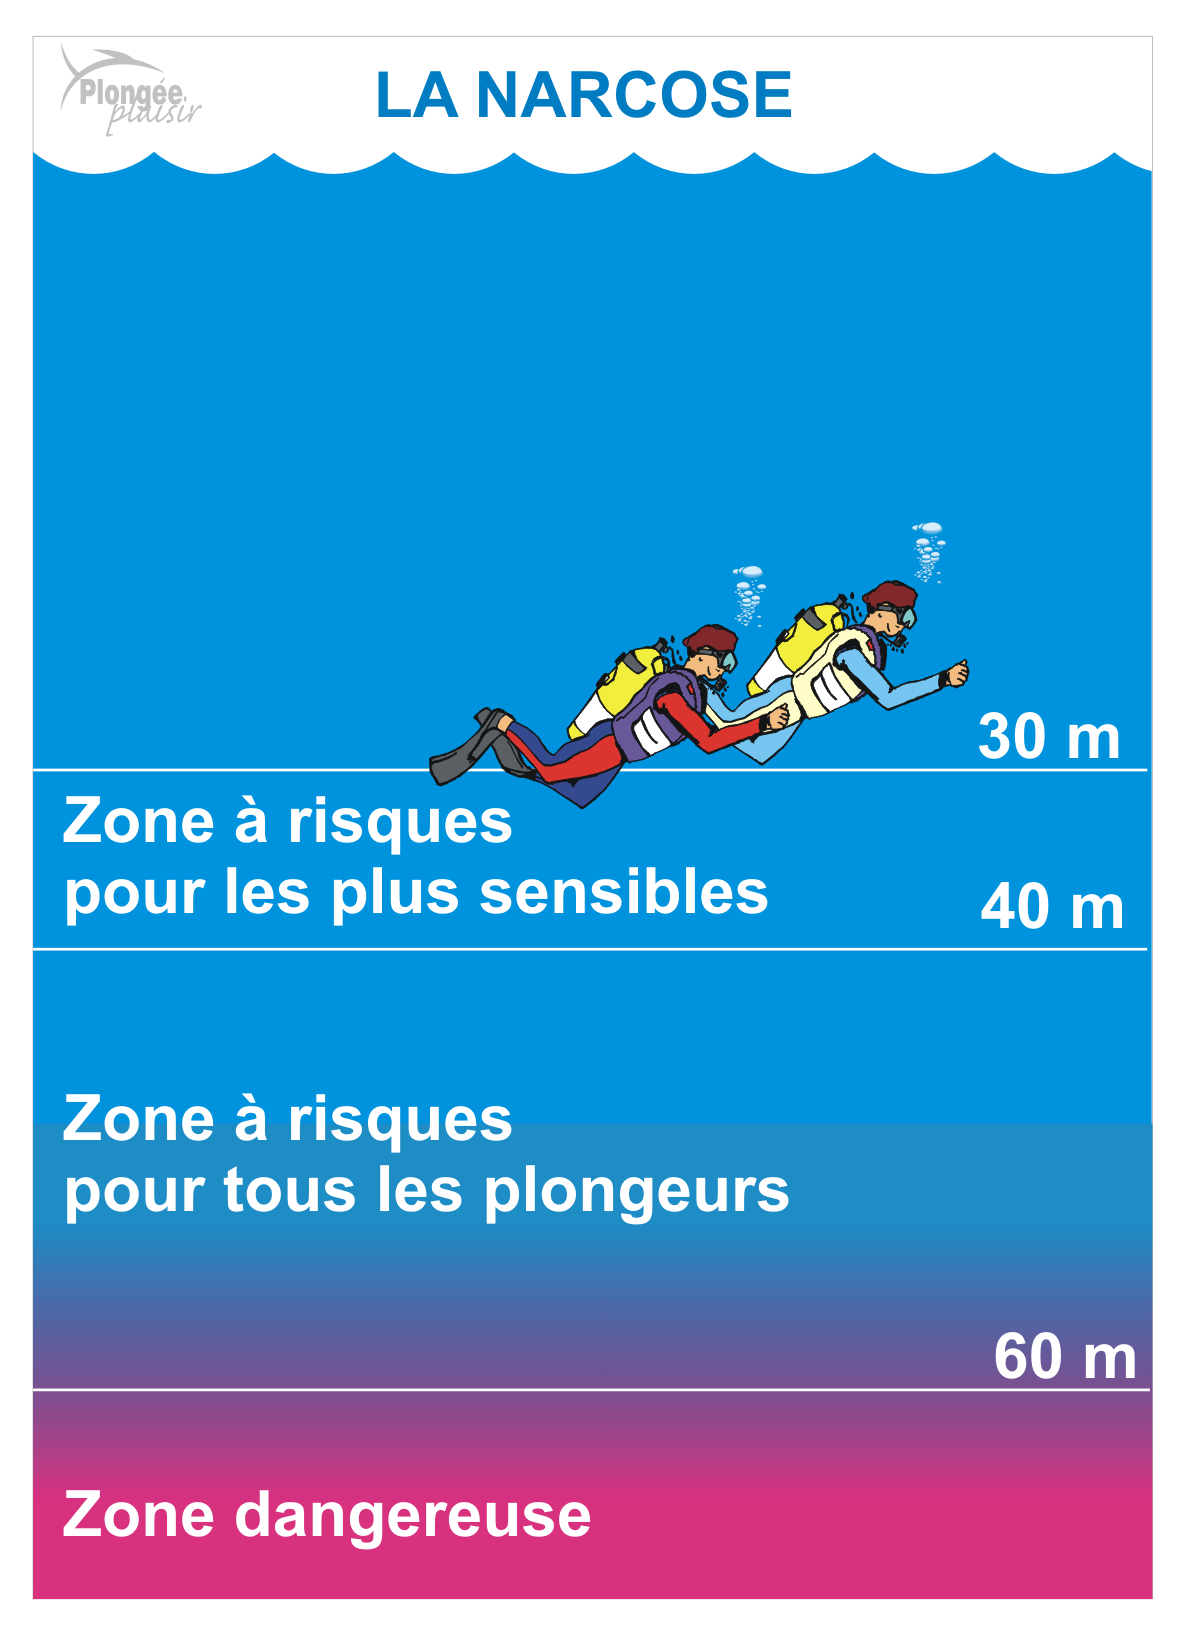
\includegraphics[height=0.85\textheight, keepaspectratio]{images/zones_narcose.png}
            \end{center}
        \end{column}
    \end{columns}
\end{frame}

\begin{frame}{Narcose — Symptômes et Signes}
    \textbf{Les Effets (souvent masqués) :}
    \begin{itemize}
        \item Troubles de la mémoire immédiate, retard de réaction, lecture répétée des instruments.
        \item Euphorie ou anxiété légère, vision tunnel.
        \item Le plongeur ne se rend souvent compte de rien.
    \end{itemize}

    \textbf{La Crise (\textcolor{ffessmred}{Danger}) :}
    \begin{itemize}
        \item Comportement aberrant (croire remonter alors qu'on descend).
        \item Incapacité à communiquer avec la palanquée.
        \item Absence de réponse aux signes.
    \end{itemize}
\end{frame}

\begin{frame}{Narcose — Prévention et CAT}
    \textbf{Prévention (Spécifique N3) :}
    \begin{itemize}
        \item \textbf{\textcolor{ffessmred}{Accès progressif}} à la profondeur (surtout en début de saison).
        \item Bonne forme physique, pas de stress, pas de médicaments.
        \item Descente \textbf{\textcolor{ffessmred}{maîtrisée}} (repères visuels).
    \end{itemize}

    \textbf{Conduite à Tenir (CAT) :}
    \begin{enumerate}
        \item \textbf{Si simples effets :} \textcolor{ffessmred}{Remonter de quelques mètres} (\textbf{10 à 15 mètres}) pour faire disparaître les troubles.
        \item \textbf{Si CRISE avérée :}
        \begin{itemize}
            \item \textbf{INTERVENTION IMMÉDIATE} du binôme.
            \item \textbf{\textcolor{ffessmred}{FIN DE PLONGÉE}} obligatoire.
            \item \textbf{Remontée assistée} vers la surface.
            \item Surveillance post-plongée (cas extrêmes).
        \end{itemize}
    \end{enumerate}
\end{frame}

\begin{frame}{L'Hypercapnie (Essoufflement) — Cause \& Mécanisme}
    \begin{columns}[T,totalwidth=\textwidth]
        \column{0.55\textwidth}
        \textbf{\textcolor{ffessmred}{Cause}} :
        \begin{itemize}
            \item Excès de \textbf{$CO_2$} (dioxyde de carbone).
            \item Souvent dû à un \textbf{effort excessif} inadapté à la profondeur ou une \textbf{mauvaise ventilation}.
        \end{itemize}

        \vspace{0.5em}
        \textbf{\textcolor{ffessmred}{Mécanisme}} :
        \begin{itemize}
            \item Augmentation du $CO_2$ dans le sang.
            \item Stimulation des centres respiratoires $\rightarrow$ besoin d'air.
            \item \textbf{Cercle vicieux} : Ventilation inefficace $\rightarrow$ $CO_2$ augmente $\rightarrow$ Fréquence s'accélère.
        \end{itemize}

        \column{0.45\textwidth}
        \centering
        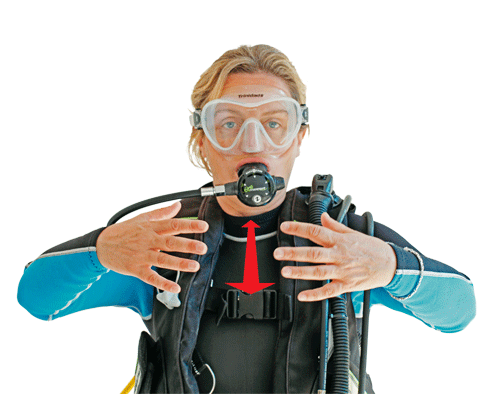
\includegraphics[height=0.7\textheight, keepaspectratio]{images/signes_essoufflement.png}
    \end{columns}
\end{frame}

\begin{frame}{L'Hypercapnie (Essoufflement) — Symptômes \& Facteurs}
    \textbf{\textcolor{ffessmred}{Symptômes}} :
    \begin{itemize}
        \item Ventilation \textbf{rapide} et \textbf{superficielle} (halètement).
        \item Sentiment d'\textbf{étouffement}, angoisse ("soif d'air").
        \item Risque de panique et d'accident grave (noyade, surpression).
    \end{itemize}

    \vspace{0.8em}
    \textbf{\textcolor{ffessmred}{Facteurs favorisants}} :
    \begin{itemize}
        \item \textbf{Matériel} : Détendeur dur/mal réglé, combinaison trop serrée.
        \item \textbf{Physique} : Froid, Stress, mauvaise condition physique.
        \item \textbf{Profondeur} : La densité de l'air augmente l'effort ventilatoire (\textit{attention à 60m !}).
        \item \textbf{Effort} : Palmage intensif contre courant.
    \end{itemize}
\end{frame}

\begin{frame}{Essoufflement — Prévention \& CAT}
    \begin{block}{Le risque associé}
        L'essoufflement augmente l'accumulation de CO$_2$ et le risque d'\textbf{ADD} 
        (accélération circulatoire $\rightarrow$ accélération ventilatoire = saturation accrue).
    \end{block}

    \vspace{0.5em}
    \begin{columns}[T,totalwidth=\textwidth]
        \column{0.48\textwidth}
        \textbf{\textcolor{ffessmred}{Prévention N3}}
        \begin{itemize}
            \item \textbf{Adapter l'effort} à la profondeur (la densité de l'air augmente).
            \item \textbf{Matériel} adapté et entretenu (détendeur, lestage).
            \item \textbf{Expiration} active et profonde.
            \item Se protéger du froid et du stress.
        \end{itemize}

        \column{0.48\textwidth}
        \textbf{\textcolor{ffessmred}{Conduite à Tenir (CAT)}}
        \begin{itemize}
            \item \textbf{\textcolor{ffessmred}{STOP}} : Arrêter tout effort immédiatement.
            \item \textbf{\textcolor{ffessmred}{Signaler}} : Prévenir le binôme.
            \item \textbf{\textcolor{ffessmred}{Ventiler}} : Se forcer à expirer à fond.
            \item Si persistant : \textbf{Assistance} et \textbf{remontée} (fin de plongée).
        \end{itemize}
    \end{columns}
\end{frame}

\begin{frame}{Essoufflement — Autonomie et adaptation au Binôme et au Milieu}
    \small
    En autonomie, l'adaptation est la clé de la sécurité.
    \vspace{0.4em}
    
    \begin{columns}[T,totalwidth=\textwidth]
        \column{0.48\textwidth}
        \textbf{Le Facteur Humain (Binôme)}
        \begin{itemize}
            \item Chaque plongeur réagit différemment (technique, condition physique).
            \item Un équipier peut se fatiguer plus vite que l'autre (souvent dû à une \textbf{\textcolor{ffessmred}{vitesse de déplacement}} excessive).
            \item \textbf{Règle} : Le rythme de la palanquée est celui du plus lent / moins expérimenté.
        \end{itemize}

        \column{0.48\textwidth}
        \textbf{Adaptation au Milieu (Courant)}
        \begin{itemize}
            \item \textbf{Surface} : Utiliser une \textbf{ligne de vie} si courant.
            \item \textbf{Immersion} : Se tenir au \textbf{mouillage} pour éviter la dérive.
            \item \textbf{Fonds} : Modifier le parcours pour s'\textbf{abriter derrière le relief}, éviter la lutte contre le courant.
        \end{itemize}
    \end{columns}

    \begin{block}{Anticipation}
        Ces stratégies doivent être définies lors du \textbf{briefing}, avant la mise à l'eau.
    \end{block}
\end{frame}